\documentclass[output=paper]{langsci/langscibook} 
\ChapterDOI{10.5281/zenodo.3975799}
\author{Alan Rumsey \affiliation{Australian National University}} 

\title{Egophoricity, engagement, and the centring of subjectivity}
%\shorttitlerunninghead{}

% \title{\texorpdfstring{Word formation and word history:\\ The case of
%  \textsc{capitalist} and \textsc{capitalism}}{Word formation and word
% history:  CAPITALIST and
% CAPITALISM}}

% \renewcommand{\lsCollectionPaperFooterTitle}{Egophoricity, engagement and the centring of subjectivity}



\abstract{In egophoric systems formal patterns that are associated with first person subjects in declarative sentences are associated with second person subjects in questions.  This difference in formal patterning is associated with a difference in the centring of subjectivity, whereby, for example, epistemic authority regarding the state of affairs that is described in a declarative sentence is vested in the speaker, whereas in a question it is vested in the addressee. Such egophoric patterning is but one instance of a wide range of phenomena that involve more-or-less regular shifts in the usual centring of subjectivity as between speaker and addressee. Here I examine three other such phenomena: 1) interactions between person marking and intentional modality; 2) shifts between speaker-centred and addressee-centred kinship terms when used in direct address; and 3) the prompting of children with utterances that are voiced as if from the child’s perspective. Evidence is drawn from the Papuan language Ku Waru and from comparison with other languages. I present an extended example of “engagement” in Ku Waru and compare it with 1-3. I show that, while grounded in the same basic aspects of human interaction, it differs from 1-3 in treating the centring of subjectivity as potentially variable, emergent,  and distributed across the interaction rather than as prototypically related to the speech roles of speaker and addressee and their alternation across speech-act types.}

\begin{document}
\maketitle

\section{Introduction}\label{s:ar1} 

In egophoric systems\footnote{In recent literature on egophoricity including the discussions of it in this volume and the detailed cross-linguistic survey in \cite{SanRoqueSchieffelin2018} that term is taken to be synonymous with what has in the past more often been called ‘conjunct-disjunct patterning’. Here I follow the above-cited literature in treating the terms as synonyms, and in using ‘egophoricity’ in preference to ‘conjunct-disjunct patterning’, noting, as do \citeauthor{SanRoqueSchieffelin2018}, that this is a distinct usage of ‘egophoric’ from that of  \cite{Hagege1974} and \citeauthor{Dahl2001} (\citeyear{Dahl2001}; \citeyear{Dahl2008}).} formal patterns that are associated with first person subjects in declarative sentences are associated with second person subjects in questions.  From a functional viewpoint this difference in formal patterning is associated with a difference in the centring of subjectivity, whereby, for example, epistemic authority regarding the state of affairs that is described in a declarative sentence is vested with the speaker, whereas in a question it is vested in the addressee.
Egophoric patterning of this kind is but one instance of a wide range of phenomena that involve more-or-less regular shifts in the usual centring of subjectivity as between speaker and addressee. In this chapter, I will examine three other such phenomena. I will compare and contrast them with egophoric patterning and ask what, if anything, is special about the latter. Evidence for my argument will be drawn from the Ku Waru language of Highland Papua New Guinea —  with particular emphasis on interactions between young children and adults —  and from comparison with other languages. The phenomena to be considered include: 1) interactions between person marking and intentional modality; 2) shifts between speaker-centred and addressee-centred kinship terms when used in direct address; and 3) the prompting of children with utterances that are voiced as if from the child’s perspective. Finally I will present an example of the nascent grammatical category of “engagement” in Ku Waru and discuss what it has in common with 1) - 3) and how it differs from them.

\section{Egophoricity}\label{s:ar2}

As a typical case of egophoricity let us consider that of Northern Akhvakh as described by \cite{Creissels2008}.   Akhvakh is a Nakh-Daghestanian language spoken in western Dagestan. It has both nominal case marking and gender-number agreement marking on the verb, both of which show ergative-absolutive alignment. Within the perfect tense/aspect Akhvakh has a formally marked distinction between the presence \textit{vs} absence of what \citeauthor{Creissels2008} calls “assertor’s involvement”. He defines the “assertor” as “the speaker in statements and the addressee in questions” (\ref{ex:rumsey:ar2}). The relevant criterion of “involvement” in Northern Akhvakh is a fully grammaticalized one: the “involved” participant is the A argument of a transitive verb or the S argument of a lexically specified subclass of intransitive verbs the subjects of which are typically volitional. This is illustrated in (\ref{ex:rumsey:ar1}) and (\ref{ex:rumsey:ar2}) by the distribution of the verb suffixes -\textit{ari} and  -\textit{ada} for +/- “Assertor’s Involvement” (\textsc{assinv})  (where “non-involvement” is signalled as the residual alternative by the Perfective suffix (\textsc{pfv}) alone).

\begin{exe}
	\ex 	\label{ex:rumsey:ar1}
	\begin{xlist}
		\ex \label{ex:rumsey:ar1a}
		\gll de-de kaʁa q̵war-\textbf{ada}.\\
		1\textsc{sg}-\textsc{erg} paper	write-\textsc{pfv}$_{\textsc{assinv}}$\\
		\trans ‘I wrote a letter.’
		\ex \label{ex:rumsey:ar1b}
		\gll me-de / hu-s̱w-e / hu-λ̱-e kaʁa q̵war-\textbf{ari}\\
		2\textsc{sg}-\textsc{erg} / \textsc{dem}-\textsc{o}$_\textsc{m}$-\textsc{erg} / \textsc{dem}-\textsc{o}$_\textsc{f}$-\textsc{erg} paper	write-\textsc{pfv}\\
		\trans ‘You / he / she wrote a letter.’
		\ex \label{ex:rumsey:ar1c} *de-de kaʁa q̵war-\textbf{ari}.
		\ex \label{ex:rumsey:ar1d} *me-de / *hu-s̱w-e / *hu-λ̱-e kaʁa q̵war-\textbf{ada}.\\ \citep[1]{Creissels2008}
	\end{xlist}
\end{exe}

\begin{exe}
	\ex 	\label{ex:rumsey:ar2}
	\begin{xlist}
		\ex \label{ex:rumsey:ar2a}
		\gll me-de čũda kaʁa q̵war-\textbf{ada}?\\
		2\textsc{sg}-\textsc{erg} when paper write-\textsc{pfv}$_{\textsc{assinv}}$\\
		\trans ‘When did you write a letter?’
		
		\ex \label{ex:rumsey:ar2b}
		\gll de-de / hu-s̱w-e / hu-λ̱-e čũda	kaʁa q̵war-\textbf{ari}?\\
		1\textsc{sg}-\textsc{erg} / \textsc{dem}-\textsc{o}$_\textsc{m}$-\textsc{erg} / \textsc{dem}-\textsc{o}$_\textsc{f}$-\textsc{erg} when paper	write-\textsc{pfv}\\
		\trans ‘When did I / he / she write a letter?’
		\ex \label{ex:rumsey:ar2c} *me-de čũda kaʁa q̵war-\textbf{ari}?
		\ex \label{ex:rumsey:ar2d} *de-de / *hu-s̱w-e / *hu-λ̱-e čũda kaʁa q̵war-\textbf{ada}?\\ \citep[1]{Creissels2008}
	\end{xlist}
\end{exe}


In a wide-ranging survey of grammatical patterning of this kind \cite[4]{SanRoqueSchieffelin2018} refer to it as \textit{egophoric distribution}. This is shown in \tabref{tab:rumsey:ar1}, which they have adapted from \cite{HaleWatters1973}, who originally interpreted egophoricity (or what they called conjunct/disjunct marking) as a kind of person marking.

\begin{table}
\begin{tabularx}{.6\textwidth}{L{.8cm}XX}
\lsptoprule& \textbf{declarative} & \textbf{interrogative}\\
\midrule
1 & \textsc{ego} & \textsc{non-ego}\\
2 & \textsc{non-ego} & \textsc{ego}\\
3 & \textsc{non-ego} & \textsc{non-ego}\\
\lspbottomrule
\end{tabularx}
\caption{Typical distribution of egophoric and non-egophoric markers with respect to person and sentence type (after \citealt[5]{SanRoqueSchieffelin2018})}
\label{tab:rumsey:ar1}
\end{table}

A complicating factor in languages that have this kind of system is that in reported speech, including indirect discourse, the egophoric marker is typically used as if grounded in the “reported” speech situation rather than the “reporting” one. An example from Akhvakh is shown in (\ref{ex:rumsey:ar3}).

\begin{exe}
	\ex \label{ex:rumsey:ar3}
	\begin{xlist}
		\ex \label{ex:rumsey:ar3a}
		\gll ha	ĩgora de-de	magazi-gune	\textbf{b-eχ-e} \textbf{j-eq’-ada}.\\
		\textsc{dem} bread 1\textsc{sg}-\textsc{erg} shop-\textsc{el}	\textsc{n}-buy-\textsc{cvb} \textsc{f}-come-\textsc{pfv}$^{\textsc{assinv}}$\\
		\trans ‘\textbf{I brought} this bread from the shop.’
		
		\ex \label{ex:rumsey:ar3b}
		\gll ilo-de$_i$ eƛ̱’-iri waša-s̱u-ga, ha ĩgora ĩ-λ̱-e$_i$ magazi-gune \textbf{b-eχ-e} \textbf{j-eq’-ada}.\\
		mother$_o$-\textsc{erg}	tell-\textsc{irr} boy-\textsc{o$_\textsc{m}$-lat} \textsc{dem} bread \textsc{ana}-\textsc{o}$_{\textsc{f}}$-\textsc{erg} shop-\textsc{el} \textsc{n}-buy-\textsc{cvb}	\textsc{f}-come-\textsc{pfv}$_{\textsc{assinv}}$\\
		\trans ‘The mother told the boy that \textbf{she had brought} this bread from the shop.’ \\ \citep[3]{Creissels2008}
	\end{xlist}	
\end{exe}


The common denominator between the reported speech cases as in (\ref{ex:rumsey:ar3b}) and the simpler, non-embedded ones as in (\ref{ex:rumsey:ar1}), (\ref{ex:rumsey:ar2}) and (\ref{ex:rumsey:ar3a}) is that egophoric marking, or what \citeauthor{Creissels2008} calls “assertor’s involvement”  marking is associated with the participant who ostensibly has what \cite{Hargreaves1991} refers to as “epistemic authority” concerning the event that is being described.  In (\ref{ex:rumsey:ar1}), (\ref{ex:rumsey:ar2}) and (\ref{ex:rumsey:ar3a}) that is the speaker in the primary speech event. In (\ref{ex:rumsey:ar3b}) it is the speaker in the reported speech event, the mother.

In most languages with egophoric marking its association with epistemic authority is overridden in certain contexts, but languages vary both in the extent to which this happens and in the contexts where it happens. One such context for some languages is rhetorical questions. This is illustrated from Akhvakh in (\ref{ex:rumsey:ar4}),\footnote{In the original source (\citealt[8]{Creissels2008}) the interlinear gloss of \textit{de-de} shows 2\textsc{sg} in initial position rather than 1\textsc{sg}. Creissels (personal communication 6 October 2016) has confirmed that this is a mistake and has corrected it in an updated version of the original Word doc file that he has kindly provided me with.} where it can be seen that in rhetorical questions the same pattern as in true questions applies, despite the fact that in the case of the rhetorical questions the addressee is not really being treated as the epistemic authority.

\begin{exe}
	\ex \label{ex:rumsey:ar4}
	\gll de-de čũda	eƛ̱’-ari	ha-be?\\
	1\textsc{sg}-\textsc{erg}	when say-\textsc{pfv} \textsc{dem}-\textsc{n}\\
	\trans 1. ‘When did I say that?’ – I don’t remember, perhaps you do (true question)\\
	2. ‘When did I say that?’ – You should know that I never did (rhetorical question) \citep[11]{Creissels2008}
\end{exe}

In other languages with egophoric marking, including Newar (\citealt[249]{HaleWatters1973}) and Awa Pit (\citealt[614--615]{Curnow2002a}), questions with first and third person subjects routinely appear with egophoric marking when they are rhetorical questions and otherwise with non-egophoric marking, which more accurately tracks the epistemic authority.
 
Another kind of variation within languages with egophoric marking is in how, and to what extent, the semantics of volitionality are taken into account as a potentially overriding factor.

This is illustrated from Newar by (\ref{ex:rumsey:ar5}).

\begin{exe}
	\ex \label{ex:rumsey:ar5}
	\begin{xlist}
		\ex \label{ex:rumsey:ar5a}
		\gll *ji pyān-ā\\
		1.\textsc{abs} be.wet-\textsc{pst}.\textsc{cj}\\
		\trans

		\ex \label{ex:rumsey:ar5b}
		\gll ji pyāt-a\\
		1.\textsc{abs} be.wet-\textsc{pst}.\textsc{dj}\\
% 		\trans ‘I got wet.’
		
		\ex \label{ex:rumsey:ar5c}
		\gll jī: (tha:-yāta) pyā-k-ā\\
		1.\textsc{erg} (self-\textsc{dat}) be.wet-\textsc{caus}-\textsc{pst}.\textsc{cj}\\
		\trans ‘I got (myself) wet.’ (\citealt[29]{Hargreaves2005})
	\end{xlist}	
\end{exe}

By contrast, within Northern Akhvakh, for any given verb there is no choice of marking its subject as either egophoric or non-egophoric in accord with its volitionality or any other contextual factor.  As Creissels puts it, “Northern Akhvakh is a nearly perfect example of a fully syntacticized system of assertor’s involvement marking, in the sense that, when the assertor of a clause in the perfective positive coincides with the A/S argument of a verb encoding a controllable event, the omission of assertor’s involvement marking is very exceptional” (\citealt[12--13]{Creissels2008}).


\subsection{Egophoric distribution and evidentiality}\label{s:ar2-1}

As will be evident from the above discussion, the kind of involvement in a predicated event or state of affairs that is deemed to be relevant for egophoric marking is typically treated as a matter of epistemic authority – the presentation of oneself as \textit{knowing about} that event or state of affairs. As was also exemplified above, a related kind of involvement that also figures in many egophoric systems is volitionality. This pertains to the difference between actions or states of affairs that have putatively been intentionally performed or brought about by the referent of the A or S argument and ones that were not under his/her control. But it is important to note that there are other linguistic phenomena which may not qualify as egophoricity \textit{per se}, but which nonetheless show the same kind of alternation in the centring of subjectivity as the one between questions and statements that is shown in \tabref{tab:rumsey:ar1}. One such area is evidentiality, as demonstrated in detail by \cite{Aikhenvald2004} and by \citeauthor{SanRoque2015} (\citealt{SanRoque2015}, \citealt{SanRoqueSchieffelin2018}), who show how it overlaps and interacts with egophoricity in that respect.  This is exemplified in (\ref{ex:rumsey:ar6}) from Duna, a Trans-New Guinea language spoken in the Southern Highlands of Papua New Guinea.

\begin{exe}
	\ex \label{ex:rumsey:ar6}
	\begin{xlist}
		\ex \label{ex:rumsey:ar6a}
		\gll ka-roko, e, no ame hutia\\
		be/stand-\textsc{sw}.\textsc{sim} hesitation 1\textsc{sg} father come.\textsc{pfv}.\textsc{vis}.\textsc{p}\\
		\trans ‘Being there, my father came (according to my visual evidence).’

		\ex \label{ex:rumsey:ar6b}
		\gll Keni hutia=pe?\\
		\textsc{psn} come.\textsc{pfv}.\textsc{vis}.\textsc{p}=\textsc{q}\\
		\trans ‘Has Kenny come? (according to your visual evidence?)’
		
		\ex \label{ex:rumsey:ar6c}
		\gll Rodni kho ayu hutia ri-tia\\
		\textsc{psn} 3\textsc{sg} now/today come.\textsc{pfv}.\textsc{vis}.\textsc{p} say-\textsc{pfv}.\textsc{vis}.\textsc{p}\\
		\trans ‘[Someone] said Rodney came today (according to their visual evidence).’ \\(\citealt[56]{SanRoqueSchieffelin2018}, from \citealt{SanRoque2008} and field notes)
	\end{xlist}	
\end{exe}

As can be readily seen from this example, the patterning of the “previous visual evidence” (\textsc{vis}.\textsc{p}) evidential category shows the same shift in the imputed knower of the evidence across statements, questions and reported speech as did the Akhvakh egophoric or “asserter’s involvement” marker in examples (\ref{ex:rumsey:ar1}), (\ref{ex:rumsey:ar2}), and (\ref{ex:rumsey:ar3}) respectively. This correspondence seems expectable (once it has been discovered!) in view of the fact that both evidentiality and egophoricity have to do with \textit{knowledge}, and the speech-act participants’ relation to it – evidentiality having to do with their \textit{sources} of knowledge and egophoricity with their \textit{presumed authority} over it or lack thereof. But interestingly, the same shift is also found with respect to other linguistic categories that pertain to another kind of “assertor involvement” besides knowledge, namely \textit{intention}. In order to illustrate this I now turn to a discussion of intentional modality, beginning with an example from Ku Waru.\footnote{As explained in \sectref{s:ar2-2}, by ‘intentional’ modality I refer to the modal categories that express an intention or desire on the part of the speaker or other relevant ‘modal subject’ (optative, imperative, hortative, etc.). I take this to be synonymous with what is sometimes also called ‘volitive’ modality, but not with ‘volitionality’ in the sense that that term is most often used by linguists, for reasons discussed below.}


\subsection{Egophoric distribution and intentional modality}\label{s:ar2-2}

Ku Waru\footnote{Ku Waru is spoken in the Western Highlands Province of Papua New Guinea and belongs to a dialect continuum that includes what Ethnologue classifies as four distinct languages: Melpa, Mbo-Ung, Imbonggu, and Umbu-Ungu. In those terms, Ku Waru belongs to the Mbo-Ung language (ISO code \textit{mux}). My collaborator Francesca Merlan and I use ‘Ku Waru’ in preference to ‘Mbo-Ung’ because it has more salience for the local people as a name for a regional speech variety. Mbo-ung, by contrast, just means ‘Indigenous language’ and does not correspond to a territorially bounded speech variety at the level of \textit{a} language.} has eight TAM categories that are indicated by verb suffixes along with seven person-number categories. One of the TAM categories is what we call the “Optative” mood. The suffixes that mark it are shown below with rough English glosses.

\begin{table}
\begin{tabularx}{\textwidth}{lll}
1\textsc{sg}	&	\textit{-ab} 	&	`I want to/intend to\_\_’	\\
2\textsc{sg}	&	\textit{-an(i)}  	&	`I want you to\_\_’, ‘Go ahead and do\_\_’	\\
3\textsc{sg}	&	\textit{-upiyl/ipiyl}	&	`Let him/her/it do\_\_’	\\
1\textsc{pl}	&	\textit{-amiyl}	&	`Let’s do\_\_’	\\
1\textsc{du}	&	\textit{-abiyl}	&	`Let’s you and I do\_\_’	\\
2/3\textsc{pl}	&	\textit{-ang}	&	`I want you (pl)/them (pl) to do\_\_’,\newline ‘You/they should do\_\_’	\\
2/3\textsc{du}	&	\textit{-angl}	&	`I want you two/those two to do\_\_’, \\
& & ‘You/they two should do\_\_’\\
\end{tabularx}
%\caption{Some good caption}
%\label{tab:rumsey:chapterhandle:keytotable}
\end{table}

Some examples of optative 1\textsc{sg} -\textit{ab} are:

\begin{exe}
	\ex \label{ex:rumsey:ar7}
	\gll na-nga wanya ly-\textbf{ab}\\
	1\textsc{sg}-\textsc{gen} hat get-\textsc{opt}:1\textsc{sg}\\
	\trans ‘I want to get my hat.’
\end{exe}


\begin{exe}
	\ex \label{ex:rumsey:ar8}
	\gll ekepu aku-na kamukamu nyi-k ti-ng ul na pily-\textbf{ab}\\
	now	that-\textsc{loc} final say-\textsc{nf}:2/3\textsc{pl}	do-2/3\textsc{pl}:\textsc{prf} thing I hear-\textsc{opt}:1\textsc{sg}\\
	\trans ‘Now I want to hear your (PL) final determination’ [lit: …hear the thing that you have said finally].
\end{exe}

\begin{exe}
	\ex \label{ex:rumsey:ar9}
	\gll ab 	ilyi ly-\textbf{ab}\\
	woman	this  get-\textsc{opt}:1\textsc{sg}\\
	\trans ‘I want to marry this woman.’
\end{exe}

When a 1\textsc{sg} optative verb is used in a question, the usual modal origo or relevant centre of intention shifts from speaker to addressee.\footnote{For a similar shift of origo in questions involving 2\textsc{sg} hortatives in another Trans-New Guinea Papuan language of the Papua New Guinea Highlands, Duna, see \citealt[448--450]{SanRoque2008}.} Examples are:

\begin{exe}
	\ex \label{ex:rumsey:ar10}
	\gll na 	lku 	suku w-\textbf{ab}-i\\
	I house	inside come-\textsc{opt}:1\textsc{sg}-\textsc{q}\\
	\trans ‘Can I come into the house?’, ‘Is it o.k. with you for me to come into the house?’
\end{exe} 

\begin{exe}
	\ex \label{ex:rumsey:ar11}
	\gll s-\textbf{ab} mola mol\\
	give-\textsc{opt}:1\textsc{sg} or no\\
	\trans ‘Shall I give [it to you] or not?’
\end{exe}

\begin{exe}
	\ex \label{ex:rumsey:ar12}
	\gll na-nga mai aprali te-k lyi-ng-lum na tena p-\textbf{ab}\\
	1\textsc{sg}-\textsc{gen} ground seize do-\textsc{nf}:2/3\textsc{pl} get-\textsc{prf}:2/3\textsc{pl}-\textsc{cond} I where go-\textsc{opt}:1\textsc{sg}\\
	\trans ‘If they take my land, where I am supposed to go? [i.e. where do you propose that I go?].’
\end{exe}

\begin{exe}
	\ex \label{ex:rumsey:ar13}
	\gll ab obi-nga aki te-pa suku pe-lym na to-p pilyi-lyo enebu to-kum pilyi-kir-ayl mel-ayl ti te-\textbf{ab} mel nar\\
	woman penis-\textsc{gen} that do-\textsc{nf}:3\textsc{sg} inside be/lie-\textsc{hab}:3\textsc{sg} I hit/do-\textsc{nf}:1\textsc{sg} know-\textsc{hab}:1\textsc{sg} tiredness hit/be-\textsc{ppr}:3\textsc{sg} know-\textsc{ppr}:1\textsc{sg}-\textsc{def}		thing-\textsc{def} another do-\textsc{opt}:1\textsc{sg} thing what\\
	\trans ‘When a woman has sex with a man that's how it is, I know; I'm an expert at it. I know it’s tiring, but what else can I do?’\footnote{This example comes from a paternity dispute, a full transcript and analysis of which is presented in \cite{MerlanRumsey1986}. In order to understand the point of this remark, it is important to know that, at least as of 1983, when the dispute took place, Ku Waru people firmly believed that is impossible for a woman to become pregnant from having sex with a man only once, multiple applications of semen being necessary to stem the flow of menstrual blood and build up the foetus. The woman who was accused of adultery in this case became pregnant at a time when she was living mainly apart from her husband, during which, as they both agreed, they had had sex between three and six times. The speaker of (\ref{ex:rumsey:ar13}) is humorously offering himself as an expert witness, attesting that in his experience it takes many more acts of intercourse to impregnate a woman than that – so many that one becomes exhausted. For the full context, see \cite[100]{MerlanRumsey1986}.}
\end{exe}
%%\footnote{This example comes from a paternity dispute, a full transcript and analysis of which is presented in Merlan and Rumsey (1986). In order to understand the point of this remark, it is important to know that, at least as of 1983, when the dispute took place, Ku Waru people firmly believed that is impossible for a woman to become pregnant from having sex with a man only once, multiple applications of semen being necessary to stem the flow of menstrual blood and build up the foetus. The woman who was accused of adultery in this case became pregnant at a time when she was living mainly apart from her husband, during which, as they both agreed, they had had sex between three and six times. The speaker of (13) is humorously offering himself as an expert witness, attesting that in his experience it takes many more acts of intercourse to impregnate a woman than that – so many that one becomes exhausted. For the full context, see Merlan and Rumsey (1986: 100).}

\begin{exe}
	\ex \label{ex:rumsey:ar14}
	\gll ab ilyi ly-\textbf{ab}-i\\
	woman this get-\textsc{opt}:1\textsc{sg}-\textsc{q}\\
	\trans ‘Do you want me to marry this woman?’, ‘Are you expecting me to marry this woman?’
\end{exe}

Now let us consider a partly comparable case from Mwotlap, an Oceanic Austronesian language of Northern Vanuatu. Mwotlap does not mark person, number or tense on the verb. It has what \citeauthor{Francois2003} (\citeyear{Francois2003}, \citeyear{Francois2004}) calls a Prospective marker \textit{so} that occurs with a wide range of modal and other meanings.  In an analysis that is consistent with other theorists of modality such as \cite{Halliday1970}, \cite{Verstraete2005} and \cite{Lehmann2012} (but different in its terminology), \citeauthor{Francois2003} (\citeyear{Francois2003}, \citeyear{Francois2004}) distinguishes between the subject of the \textit{modus} (i.e., of the modal projection encoded by the Prospective marker) and the subject of the \textit{dictum} (of the sentence itself). While the latter is explicitly encoded within the sentence, the subject of the \textit{modus} is left unspecified, and must be retrieved from the context. There are certain default patterns to this inference, one of which relates to the difference between declarative sentences and questions. Let us first consider a declarative example, as provided to me by François (personal communication March 12, 2016) based on one of the examples in \cite[221]{Francois2003}.

\begin{exe}
	\ex \label{ex:rumsey:ar15}
	\gll Nok so leg mi kē.\\
	1\textsc{sg} \textsc{prosp} marry with 3\textsc{sg}\\
	\trans ‘I <Prosp> marry her.’
\end{exe}

Here are possible readings given to me by \citeauthor{Francois2003} for (\ref{ex:rumsey:ar15}) as a statement:

\begin{enumerate}[label=\alph*)]
	\item \label{ex:rumsey:ar15a} \textbf{I want to} marry her\\modal subject = Speaker
	\item \label{ex:rumsey:ar15b} \textbf{I am being asked to} marry her\\modal subject =  a specific person with the authority to impose my future wife upon me:  my father, 				or uncle, etc.)
	\item \label{ex:rumsey:ar15c} \textbf{I am supposed to} marry her\\modal subject = an impersonal custom  (e.g., if marriage rules mean that I should marry that woman rather than another one)
	\item \label{ex:rumsey:ar15d} \textbf{I was supposed to} marry her / should have married her\\modal subject = an authority, whether specific (father+) or non-specific (custom…)… but with retrospective reading
	\item \label{ex:rumsey:ar15e} \textbf{I'm going to} marry her\\non-modal readings e.g. typically in a dependent clause: `She will move to my village, that's because I'll be marrying her…'
	\item \label{ex:rumsey:ar15f} \textbf{If/When} I marry her…\\ suspended modal origo (yielding a conditional protasis)
\end{enumerate}

Here are possible readings given by \citeauthor{Francois2003} for that same sentence with question intonation:

\begin{exe}
	\ex \label{ex:rumsey:ar16}
	\gll Nok so leg mi kē?\\
	1\textsc{sg} \textsc{prosp} marry with 3\textsc{sg}\\
	\trans ‘I <Prosp> marry her?’

\begin{xlist}
	\ex\label{ex:rumsey:ar16a} \textbf{May I} marry her? \\modal subject = Addressee (asking for permission, e.g., to own father)
	\ex\label{ex:rumsey:ar16b} \textbf{Do you think I should} marry her? \\modal subject = Addressee (asking for advice, e.g., if confiding to my friend, asking them whether they think this is the right choice for me)
  	\ex\label{ex:rumsey:ar16c} \textbf{Am I supposed to} marry her? \\modal subject = an authority, whether specific (father+) or non-specific (custom…) François adds:\\ “For example, if I confide to my uncle who knows well how custom or kinship systems or marriage rules work, and assuming I want to do well to please my extended family and marry the `righ' person, then the modal origo would not be my addressee, but rather, a diluted, perhaps impersonal subject, whatever we understand as `custom' (as it is often called in Melanesia) or `law' (as among indigenous Australians)…” [cf. \citealt[229]{Francois2003}]
  	\ex\label{ex:rumsey:ar16d} \textbf{Am I going to} marry her? \\ non-modal readings (assuming there's a context where one could ask this question with no particular feelings or modal contents, as in: `What's the plan exactly? Will I marry her?")
\end{xlist}
\end{exe}

These uses of Prospective marking in Mwotlap compare interestingly with those of the optative mood in Ku Waru as discussed above. The main difference is that the uses of the latter are much more wide-ranging than the former. To see this, compare Ku Waru example (\ref{ex:rumsey:ar9}) with Mwotlap example (\ref{ex:rumsey:ar15}). As can be seen, (\ref{ex:rumsey:ar9}) has the same sense as the one given for Mwotlap in (\ref{ex:rumsey:ar15}\ref{ex:rumsey:ar15a}.  But it cannot express non-modal meanings (as in \ref{ex:rumsey:ar15}\ref{ex:rumsey:ar15e} or any of the other modal ones in  (\ref{ex:rumsey:ar15}\ref{ex:rumsey:ar15b}--(\ref{ex:rumsey:ar15}\ref{ex:rumsey:ar15d}, all of which are expressed in other ways in Ku Waru. But notwithstanding this difference, when Mwotlap \textit{so} does express a modal meaning, it shows the same crossover between speaker- and addressee-centred modality in questions as opposed to statements. This is shown in \tabref{tab:rumsey:ar2}, which is reproduced from \cite{Francois2003} with the title shown in English. (Note that “C\textsubscript{én}” in the top row stands for “centre énonciative”, or “modal subject” as \citeauthor{Francois2003} renders it in the examples above.)

\newcommand{\rumseymark}[1]{\hspace*{-1mm}\tikz[remember picture]\node(#1)[inner sep=0mm]{};}

%%TODO table 2
\begin{table}
% 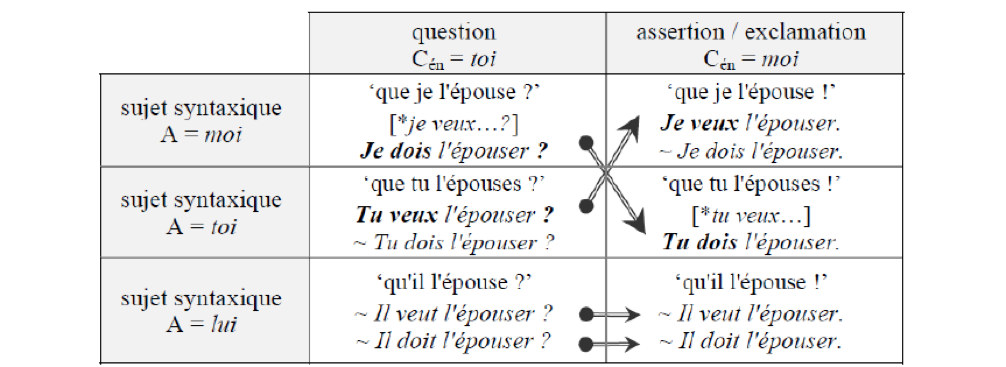
\includegraphics[width=\linewidth]{figures/rumsey_tab2.png}
\begin{tabularx}{\textwidth}{CQQ}
% \cline{2-3}
\lsptoprule
   & question& assertion/exclamation\\
   & \itshape C\textsubscript{én}=toi & \itshape C\textsubscript{én}=moi \\
% \hline
\midrule
sujet syntaxique\newline \itshape A=moi &
    `que je l'épouse ?'\newline
    [*\textit{je veux {\dots}?}]\newline
    \textit{\textbf{Je dois} l'épouser \textbf{?}}\rumseymark{moitoi} &
        `que je l'épouse !'\newline
        \textit{\textbf{Je veux} l'épouser.}\newline
        \rumseymark{moimoi}\textasciitilde\textit{Je dois l'épouser.}\\

\tablevspace
\tablevspace
sujet syntaxique\newline\itshape A=toi &
    `que tu l'épouses ?'\rumseymark{toitoi}\newline
    \textit{\textbf{Tu veux} l'épouser \textbf{?}}\newline
    \textasciitilde\textit{Tu dois l'épouser ?} &
        \rumseymark{toimoi}`que tu l'épouses !'\newline
        [*\textit{tu veux {\dots}}]\newline
        \textit{\textbf{Tu dois} l'épouser.} \\
\tablevspace
\tablevspace
sujet syntaxique\newline \itshape A=lui &
    `qu'il l'épouse ?'\newline
    \textasciitilde\textit{Il veut l'épouser \textbf{?}}\rumseymark{luitoi1}\newline
    \textasciitilde\textit{Il doit l'épouser \textbf{?}}\rumseymark{luitoi2} &
        `qu'il l'épouse !'\newline
        \rumseymark{luimoi1}\textasciitilde\textit{Il veut l'épouser.}\newline
        \rumseymark{luimoi2}\textasciitilde\textit{Il doit l'épouser.}\\
% \hline
\lspbottomrule
\end{tabularx}

\begin{tikzpicture}[overlay,remember picture]
\draw[->, black, thick] (moitoi)->(toimoi);
\draw[->, black, thick] (toitoi)->(moimoi);
\draw[->, black, thick] (luitoi1)->(luimoi1);
\draw[->, black, thick] (luitoi2)->(luimoi2);
\end{tikzpicture}

\caption{The crossover between volitive and deontic values of the Prospective in Mwotlap (after \citealt[228]{Francois2003})}
\label{tab:rumsey:ar2}
\end{table}

The correspondence between the crossover in \tabref{tab:rumsey:ar2} and that in \tabref{tab:rumsey:ar1} is striking, especially in view of the fact that \citeauthor{SanRoqueSchieffelin2018}’s table is presented as pertaining to egophoricity and evidentiality with no reference to modality, and \citeauthor{Francois2003}’ table as pertaining to modality with – so he tells me – no thought of its possible relevance for any other grammatical domain at the time when he produced it (personal communication March 25, 2016).

While this kind of crossover has become almost definitional of egophoricity or “conjunct/disjunct” marking, and also has been recognized with regard to evidentiality as discussed above, it has seldom been noted with respect to modality, which has generally been treated as if it were exclusively speaker-centred. Besides \citeauthor{Francois2003} (\citeyear{Francois2003}, \citeyear{Francois2004}), the main exception that I am aware of is \cite{Lehmann2012}, who develops a systematic typological comparison among six languages in this respect, and on that basis argues for an overarching category of “subjective” modality which includes, for all six of the languages, modal categories within which such interrogative-declarative crossover is found.

I have developed the Ku Waru - Mwotlap comparison in particular here for two reasons.  The first is that, although the examples I presented from those languages are in full accord with the “egophoric distribution” shown in \tabref{tab:rumsey:ar1}, they fall outside the scope of most of the existing literature on egophoric systems, almost all of which is exclusively concerned with the role in grammar of \textit{epistemic} authority or involvement. In other words, the “ego” in “egophoric” is taken to be a \textit{knowing} ego and the relevant asymmetries among speech act participants are taken to be ones of knowledge. By contrast, the relevant semantic considerations here are ones of deontic or intentional modality – what the entailed ego \textit{wants}, or what others want of him/her.

The other reason for my comparison between Ku Waru and Mwotlap is that I think it shows with particular clarity how patterns that are fully grammaticalized in one language may be evident in the discourse patterning of another. In the following section, I build on that by moving beyond the semantics and pragmatics of egophoricity, evidentiality and modality to other aspects of language use that do not show the same pattern of crossover between speaker and addressee, but which are similar to the above examples insofar as they involve more-or-less regular shifts in the usual centring of subjectivity as between speaker and addressee.  Arising as they do from my current work on child language socialization, a common factor among these remaining examples is that they all involve speech that is addressed to young children.

\section{Altercentric kin term usage}\label{s:ar3}

There are at least two ways in which Ku Waru adults’ use of kin terms to children differs from their usage to other adults, and from children’s use of them to anybody. The first of these is what \cite{Merlan1982} in an Australian context dubbed “altercentric usage”. To understand what that involves, it is helpful to introduce the term “anchor” as used by \cite{DahlK-T2001}. For any given kin term within a given context, the anchor is the person or persons from whom the relevant relation is reckoned. So for example the anchors of “Fred’s uncle”, “our aunt”,  and “Daddy”, when used by a child to her father, are “Fred”, 1\textsc{pl} and 1\textit{sg}  respectively. Usually when kin terms are used without explicit reference to an anchor, the implicit anchor is the speaker as in the “daddy” example above. But alternatively it may be the addressee, as for example when a mother says to a child “Give it to Mommy” or “Where’s Daddy?”. What \cite{Merlan1982} drew attention to was: 1) that this phenomenon, which she called “altercentric” usage, is very common around the world; 2) that it is especially common in speech addressed to young children by adults and older children; and 3) it is typically non-reciprocal, i.e., it is used when children are being addressed by adults but not vice versa.\footnote{For further elaboration of this typology including other kinds of anchor-shift and examples of them see \cite{Agha2006}.} 

Altercentric usage of kin terms is common in Ku Waru, and is in accord with Merlan’s generalizations. Examples are:

\begin{exe}
	\ex \label{ex:rumsey:ar17}
	\gll ma tena pu-m\\
	mommy where	go-\textsc{prf}:3\textsc{sg}\\
	\trans ‘Where did [your] mommy go?’  (Said by a father to his 2\textonehalf{} year old son)
\end{exe}

\begin{exe}
	\ex \label{ex:rumsey:ar18}
	\gll tata uj me-ba o-kum\\
	daddy wood carry-\textsc{nf}:3\textsc{sg} come-\textsc{ppr}:3\textsc{sg}\\
	\trans ‘[Your] daddy is bringing firewood.’ (Said by a mother to her 3-year old daughter).
\end{exe}

\begin{exe}
	\ex \label{ex:rumsey:ar19}
	\gll ana apu tupily\\
	same.sex.sibling carry.on.shoulder hit/do:\textsc{opt}:3\textsc{sg}\\
	\trans ‘Let your sister carry you on her shoulder.’ (Said by woman to her 2\textonehalf{} year old niece)
\end{exe}

Note that in all these examples (as in the English examples of altercentric usage above) there is no explicit indication of the anchor. Just as in the English examples, it would have been possible to include one, with a possessive pronoun ‘your’ (\textit{nunga}). But in both cases, as in many other attested ones from around the world, that indication of the anchor tends to be left out in altercentric kin-term usage by adults to children. 	

Another thing to note is that in both the English case and the Ku Waru one (again, as is common around the world), the kin terms that are used in this way are ones that in other contexts are characteristically used by children: “daddy” and “mommy” rather than “(my) father”, “(my) mother”, etc. Likewise in Ku Waru the terms \textit{ma}, \textit{tata} and \textit{ana} are ones that are in other contexts used more by children than adults. 

I suggest that what is going on here bears a family resemblance to what we saw above regarding the shift of typical modal origo as between statements and questions in egophoric, evidential and modal contexts, in two ways. First, in both cases the shift is between Speaker and Addressee as the relevant implicit ground in relation to which the meaning is figured.  Second, in both cases this happens within a specific context: questions \textit{vs} statements in the case of the modal shift and speech by adults to young children \textit{vs} other adults and older children in the case of kin term usage. Another similarity is that the shifts in question are very widely attested in the languages and speech communities of the world. Below I will address the question of why this should be the case. First I will introduce another kind of shift that is widely found in the use of kin terms to children.

\section{“Address inversion”}\label{s:ar4}

In examining transcripts of interactions involving Ku Waru children one thing I have been struck by is a regular pattern whereby an adult when speaking to a child addresses him/her with the kin term that the child uses when addressing that adult. So for example a man addresses his (“actual” or classificatory) son or daughter by a term that ordinarily means ‘daddy’, and addresses his nephew or niece by a term that ordinarily means ‘uncle’.  Examples are:

\begin{exe}
	\ex Man to his “daughter”\footnote{The ‘daughter’ who is being addressed here is in European terms not the speaker’s own daughter, but the daughter of one of his ‘classificatory’ brothers, which in Ku Waru (as in many languages) places her in the same kin category as his own daughter (\citealt{Kroeber1909}). Similar considerations apply to the kin relations in examples  (\ref{ex:rumsey:ar21})--(\ref{ex:rumsey:ar23}).} (age 3):\label{ex:rumsey:ar20}\\
	\gll papa=o nu ur nai-kin pin?\\
	daddy=\textsc{voc} 2\textsc{sg}	sleep who-\textsc{com} be/lie:\textsc{prf}:2\textsc{sg}\\
	\trans ‘Daddy [i.e., daughter], with whom did you have a sleepover?’
\end{exe}
%%\footnote{The ‘daughter’ who is being addressed here is in European terms not the speaker’s own daughter, but the daughter of one of his ‘classificatory’ brothers, which in Ku Waru (as in many languages) places her in the same kin category as his own daughter  (\citealt{Kroeber1909}). Similar considerations apply to the kin relations in examples  (\ref{ex:rumsey:ar21})--(\label{ex:rumsey:ar23}).}

\begin{exe}
	\ex Man to his niece (age 3 ½):\label{ex:rumsey:ar21}\\
	\gll angkol=o nu pu-ni mola mol\\
	uncle=\textsc{voc} 2\textsc{sg} go-\textsc{fut}:3\textsc{sg} or no\\
	\trans ‘Uncle [i.e. niece], are you going or not?’
\end{exe}

\begin{exe}
	\ex Man to his son	(age 4)	:\label{ex:rumsey:ar22}\\
	\gll papa e mel kuduyl ilyi kana-kin-i\\
	daddy hey thing red this see-\textsc{ppr}:2\textsc{sg}-\textsc{q}\\
	\trans ‘Hey Daddy [i.e., son], do you see this red thing?’
\end{exe}

\begin{exe}
	\ex \label{ex:rumsey:ar23}
	\begin{xlist}
	\ex John, to his daughter (age 3):\label{ex:rumsey:ar23a}\\
	\gll ep na-nga oma mari tuju-ni?\\
	now 1\textsc{sg}-\textsc{gen} fish some hit:\textsc{ben}-\textsc{fut}:2\textsc{sg}\\
	\trans ‘Now will you catch some fish for me?’ 	
	
	\ex Saina (the girl’s mother):\label{ex:rumsey:ar23b}\\
	\gll toju-ba-yl\\
	hit:\textsc{ben}-\textsc{fut}:3\textsc{sg}-\textsc{def}\\
	\trans ‘Indeed she will.’
	
	\ex John:\label{ex:rumsey:ar23c}\\
	\gll e? a na-nga papa-n…\\
	really? oh 1\textsc{sg}-\textsc{gen} daddy-\textsc{erg}\\
	\trans ‘Really? Oh, my ‘daddy’ [i.e., daughter] [will catch some]
	\end{xlist}
\end{exe}

In all these examples, in place of the junior term within a given dyad (father-daughter, uncle-niece, father-son) the senior term is used in address and reference to the junior member of the pair, regardless of his or her gender. Although such usage may seem unusual from an Anglophone perspective, it is actually quite widely attested from elsewhere in the world, including Albanian, Arabic, Bengali, Bulgarian, Greek, Hungarian, Italian, Norwegian, Persian, Romanian, Russian, Tok Pisin, Turkish and many other languages where it has been documented under the rubrics of \textit{allocuzione inversa} (\citealt{Renzi1968}), \textit{umgekehrte Anrede} (\citealt{BeyerKostov1978}), and “address inversion” (\citealt{Braun1988}).  This is actually a misnomer, for two reasons.  The one that is especially relevant here is that, as shown by Braun, in the great majority of attested practices of this kind, there is actually not a full inversion. That is, while the senior party uses the term for the junior one that the latter uses for him or her, the junior party does not change his or her usage in the opposite direction. For example the man’s classificatory daughter in example (\ref{ex:rumsey:ar20}) does not reciprocate by calling him by a term for “daughter”. Nor does the man’s son in (\ref{ex:rumsey:ar22}) call his father “son”. Rather the children continue to call him by a father term. 

What are we to make of these usages? As different as they are from the altercentric ones discussed above, there are, I suggest, three important similarities:

\begin{enumerate}
	\item Both are associated with speech by adults to young children.
	\item Both involve a shift of perspective that is made by the adult when addressing the child, but not by the child in return.
	\item In both cases the perspective that is taken is that of the child, or one that assimilates to it.\label{similarity3}
\end{enumerate}

That \ref{similarity3} is true in the case of altercentric kin term usage should be obvious. It is also true of “address inversion” insofar as the terms that are used, even as their reference is reversed, are ones that are normally used by children to adults, just as in the altercentric case. But why the apparent reversal of reference?  Friederike \citet{Braun1988} has suggested that “the senior [kin term] used for inversion could be regarded as an archilexeme referring to the dyad as a whole, though explicitly naming only one of its partners”\footnote{In that respect ‘address inversion’ is like ‘dyadic’ kin terms such as discussed by \cite{MerlanJeffrey1982} and \cite{Evans2006a}. Dyadic kin terms are ones which refer to a pair of people who stand in a given relationship to each other. They mean things like ‘pair of brothers’, ‘mother and child’, etc.  There is a widespread pattern found among those terms, first pointed out by \cite{MerlanJeffrey1982}, such that whenever they are based on the word for one member of an intergenerational pair such as father-son, uncle-nephew, etc., it is the term for the senior member that becomes the basis for the dyadic term. For example in Kayardild, an Australian Aboriginal language spoken on the South Wellesley Islands of Northern Queensland, such terms are formed with a dyadic suffix –\textit{ngarrba}; the expression for "mother and child", \textit{ngamathu-ngarrba}, is formed by combining this suffix with the word for ‘mother’, \textit{ngamathu}. Likewise in Icelandic the dyadic terms \textit{feðgin} "father and daughter" and \textit{mæðgin} ‘mother and son’ are derived from the words for ‘father’ and ‘mother’ respectively (\citealt{Evans2006a}).} (\citealt[285]{Braun1988}). I’m not sure how well that proposal could be supported on formal grounds in the Ku Waru case, but in functional terms there does seem to me to be something right about the idea that the “inverse” uses of kin terms highlight the relationship \textit{per se}. And in Ku Waru and elsewhere it seems to me no accident that the terms which do that, and which shift the anchor from speaker to addressee, should be particularly associated with contexts in which adults are speaking to children. For the highlighting of relationships is one of the main ways in which children are socialized and culture is transmitted.

\section{Prompting routines}\label{s:ar5}

I now turn to a much more general phenomenon involving the same kind of transposition of perspectives as in the use of altercentric kin terms. This is the phenomenon of prompting, i.e., of adults presenting utterances to the children for them to repeat to others.\footnote{For extensive discussion and exemplification of prompting in Kaluli, a Papuan language spoken in the Bosavi region about 120 km to the southwest of Ku Waru see \cite{Schieffelin1990}. For cross-culturally comparative accounts of this very widespread phenomenon see \cite{Demuth1986} and \cite{Moore2012}.} An example is shown in (\ref{ex:rumsey:ar24}). This bit of conversation took place at Kailge, a settlement which lies at the end of a long and winding unpaved road about one hour’s ride from Mount Hagen, the capital of Western Highlands province. The speakers were a man named Taka and his eighteen-month old daughter Laplin. Both of them were looking at an older boy named Mawa who was passing by.

\begin{exe}
	\ex \label{ex:rumsey:ar24}
	\begin{xlist}
	\ex Father:\label{ex:rumsey:ar24a}\\
	\gll mawa wi to\\
	{(boy’s name)} call.out.to do:\textsc{imp}:\textsc{sg}\\
	\trans ‘Call out to Mawa.’ 	
	
	\ex Daughter [shouts]:\label{ex:rumsey:ar24b}\\
	mawai!\\
	\trans ‘Hey Mawa!’
	
	\ex Father:\label{ex:rumsey:ar24c}\\
	\gll kar-na p-abiyl wa! kar!\\
	truck-\textsc{loc} go-\textsc{opt:1du} come:\textsc{imp:sg} truck\\
	\trans ‘Come, let’s you and me go in the car! The car!’
	
	\ex Daughter:\label{ex:rumsey:ar24d}\\
	\gll wa\\
	come:\textsc{imp}:\textsc{sg}\\
	\trans ‘Come!’
	\end{xlist}
\end{exe}

The father’s utterance in line c is a typical instance of prompted speech in that it is voiced from his daughter’s point of view, for her to repeat. Sometimes such prompts are explicitly framed with the imperative form of the word for ‘say’ (\textit{nya}), but more often they are not, as in this case. The daughter nonetheless understands this as a prompt, and responds appropriately. She is at the one-word stage of language acquisition, so her father’s utterance with its concatenated first person dual optative verb and locative-marked accompanying NP is far too complex for her to understand and repeat in its entirety, but she nonetheless understands that it is a prompt, picking out its most central element, the imperative verb \textit{wa} ‘come’, and repeating it as if from her own viewpoint.

Another, more complex example of prompting is shown in 25. This is from a conversation between a Ku Waru mother (Wapi) and her two-year-old son (Jesi), in the presence of his five-year-old brother Alex.\footnote{ For some of the son’s utterances in this transcript there are two parallel lines of Ku Waru. The first line shows what he actually said and the line below it shows what our Ku Waru-speaking transcription assistant has offered as an adult equivalent of that utterance.  For further discussion of this interaction see \cite{Rumsey2014}.}

\begin{exe}
	\ex \label{ex:rumsey:ar25}
	\begin{xlist}
	\ex Mother:\label{ex:rumsey:ar25a}\\
	\gll ana kola naa ti=o nya\\
	same.sex.sibling cry not do:\textsc{jus}=\textsc{voc} say:\textsc{imp}:\textsc{sg}\\
	\trans ‘Tell your brother not to cry [lit: ‘Say “brother, don’t cry”’]’ 	
	
	\ex Son:\label{ex:rumsey:ar25b}\\
	\gll ana kola naa ti=o\\
	same.sex.sibling cry not do:\textsc{jus}=\textsc{voc}\\
	\trans ‘Brother don’t cry.’
	
	\ex Mother:\label{ex:rumsey:ar25c}\\
	\gll kali p-abiyl=o\\
	kalyke go-\textsc{opt}:2\textsc{du}=\textsc{voc}\\
	\trans ‘Let’s go to Kailge.’
	
	\ex Son:\label{ex:rumsey:ar25d}\\
	\glll teka pabi=o\\
	kalyke p-abiyl=o\\
	Kailge go-\textsc{opt}:2\textsc{du}=\textsc{voc}\\
	\trans ‘Let’s go to Kailge.’
	
	\ex 	Mother: \label{ex:rumsey:ar25e}\\
	\gll sispop ly-abiyl p-abiyl=o\\
	cheesepop get-\textsc{opt}:2\textsc{du} go-\textsc{opt}:2\textsc{du}=\textsc{voc}\\
	\trans ‘Let’s go get some cheesepops.’
	
	\ex Son:	\label{ex:rumsey:ar25f}\\
	\glll titopa-ti nabi\\ 
	sispop-ti n-abiyl\\
	cheesepop-\textsc{idf} eat-\textsc{opt}:2\textsc{du}\\
	\trans ‘Let’s eat a cheesepop.’
	
	\ex Mother:\label{ex:rumsey:ar25g}\\
	\gll p-abiyl\\
	go-\textsc{opt}:2\textsc{du}\\
	\trans ‘Let’s go.’
	
	\ex Son:\label{ex:rumsey:ar25h}\\ 
	\glll pebil=o\\
	p-abiyl=o\\
	go-\textsc{opt}:2\textsc{du}=\textsc{voc}\\
	\trans ‘Let’s go.’
	
	\newpage
	\ex Mother:\label{ex:rumsey:ar25i}\\
	\gll kola naa ti=o\\
	cry not do:\textsc{jus}=\textsc{voc}\\
	\trans ‘Don’t cry.’
	
	\ex Son:\label{ex:rumsey:ar25j}\\
	\gll pike naa ti\\
	bighead not do:\textsc{jus}\\
	\trans ‘Don’t be a bighead (disobedient).’
	\end{xlist}
\end{exe}

\largerpage
All of the mother’s utterances in this example are prompts offered to her son for him to repeat. Only the first one (\ref{ex:rumsey:ar25a}) is explicitly framed as such by the imperative verb \textit{nya} ‘say’. But again the son understands them all as prompts and responds appropriately. In lines (\ref{ex:rumsey:ar25b}), (\ref{ex:rumsey:ar25d}), (\ref{ex:rumsey:ar25f}) and (\ref{ex:rumsey:ar25h}) he does this by repeating the utterances he has been prompted to say (sometimes in his own toddler-talk variants). In line (\ref{ex:rumsey:ar25j}) he responds more creatively by saying something that does not repeat the prompt verbatim but is fully within the spirit of it, chastising his brother for being a “bighead”. The framing relationship between the mother’s prompt in line (\ref{ex:rumsey:ar25a}) and the prompted response that she projects for her son in it is shown in \figref{fig:ar1}. The sons’s response in line (\ref{ex:rumsey:ar25b}) and all of his subsequent ones are interactionally complex in that they are positioned both as responses to his mother and as injunctions directed to his brother Alex. The same is true of the daughter’s responses to her father in \ref{ex:rumsey:ar24}. In interactional terms, the utterances by the parents that prompt these responses are similar to what happens with altercentric kin term usage as exemplified above, in that the adult speaker is in effect aligning his or her perspective with that of the child, while at the same time retaining his/her position as the controlling party from whose perspective the child’s utterance is projected.\footnote{A reviewer comments regarding this form of prompting that it ‘seems to be very different from the perspective shift in altercentric kinship terms. Here the ``perspective shift'' is a natural consequence of the fact that the prompt is given verbatim, as direct (pre-)reported discourse, which is the simplest way to instruct a child what to say.’ I agree that prompting is different in kind from altercentric kinterm usage in that it is in some instances explicitly marked as what the referee calls ‘direct (pre-)reported discourse’. But in those many instances where it is \emph{not} explicitly framed in that way by a verb of saying, it is more like altercentric kinterm usage in that the shift of perspective (or, in \citeauthor{Buhler1990}’s \citeyear{Buhler1990} terms, transposed origo) must be indirectly inferred by the addressee, in this case the child. I suggest that the children’s ability to do that so readily from a very early age results in part from the regularity of the direction in which that shift takes place, as identified in the following sentence.} Accordingly, in common with altercentric kin term usage, the projection of perspectives within prompting routines is asymmetrical in that it is always done by the adult in relation to the child, never the other way around.
\clearpage

%TODO figure 1
\begin{figure}
\centering
% 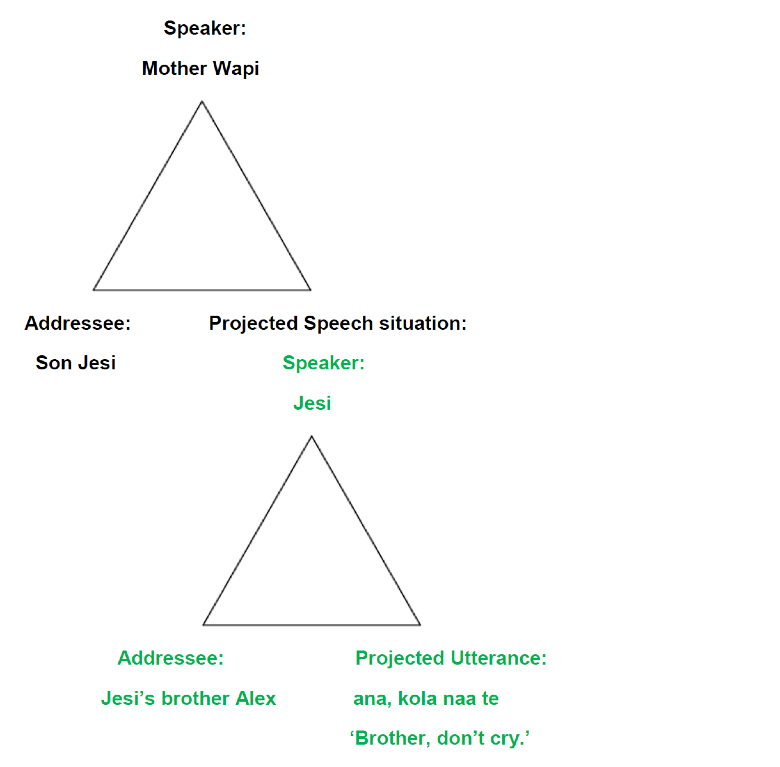
\includegraphics[width=8cm]{figures/rumsey-fig1.png}
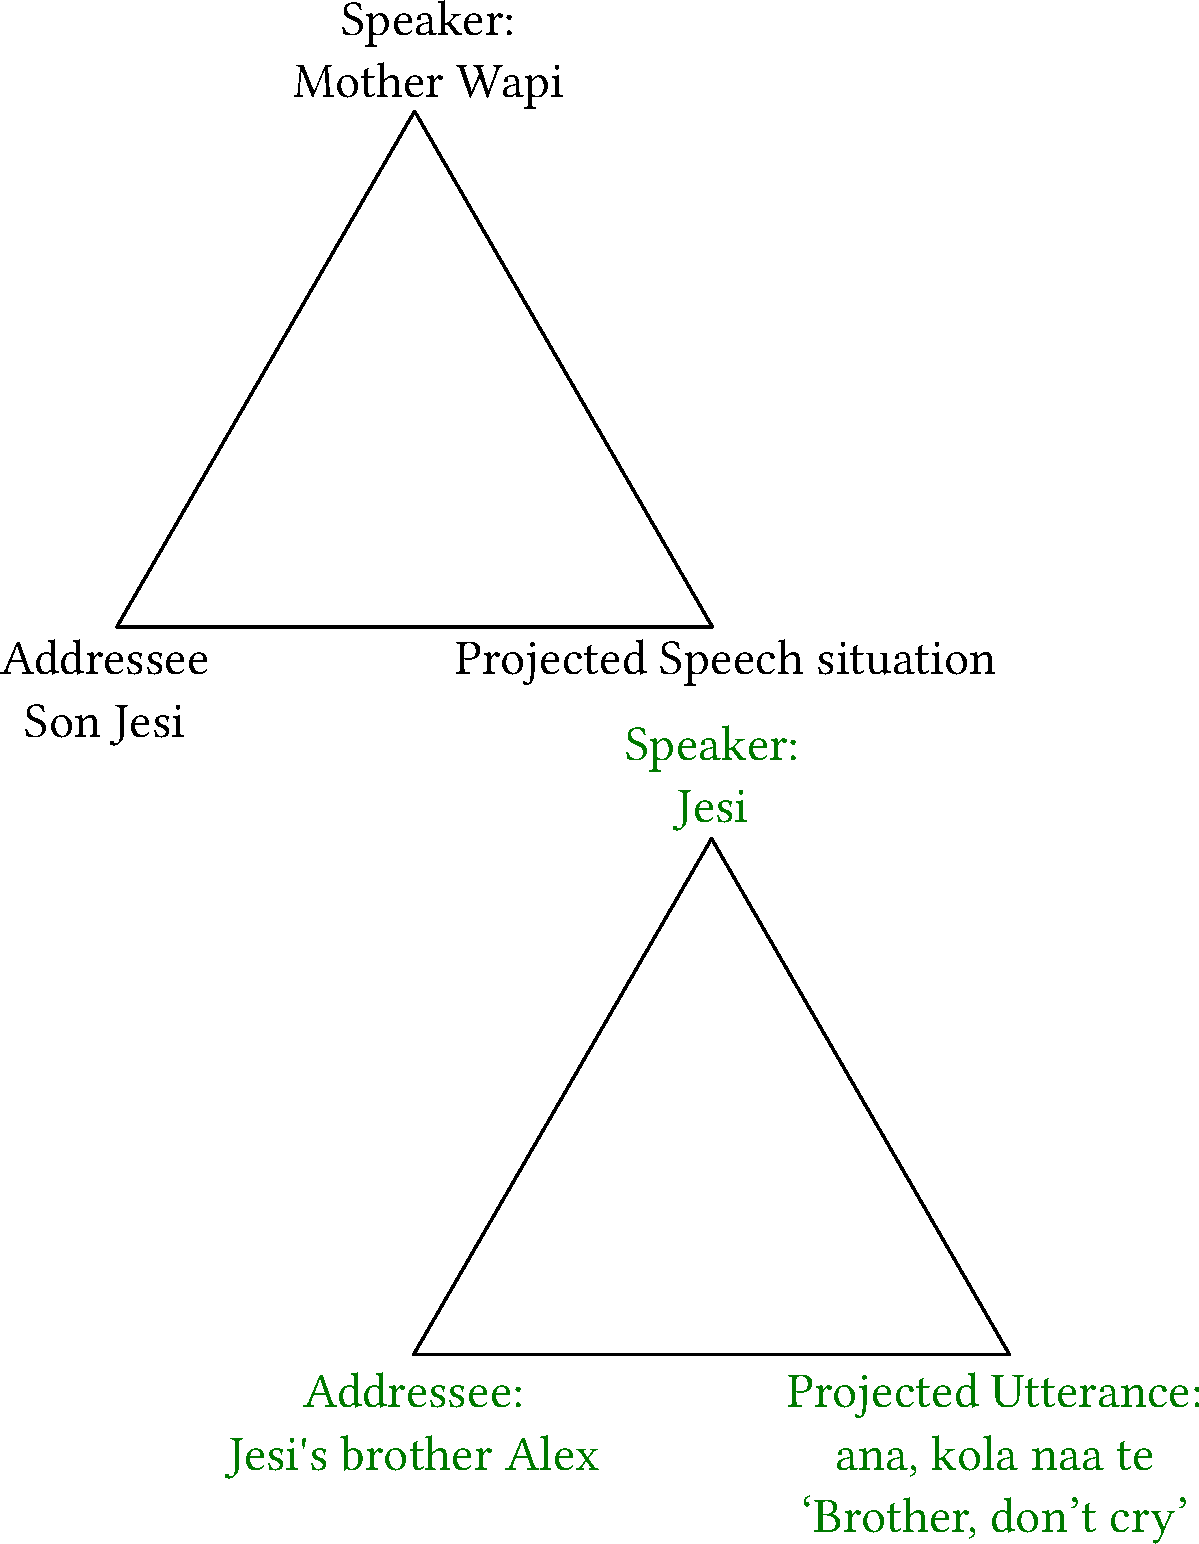
\includegraphics[height=.4\textheight]{figures/rumsey-wapijesi.pdf}
 \caption{Interactional framing in conversation between Wapi and Jesi} 
 \label{fig:ar1}
\end{figure}


\section{Discussion}\label{s:ar6}

In the first part of this chapter I have discussed the regular shifts in the centring of subjectivity as between speaker and addressee that are entailed in the use of the grammatical categories of egophoricity, evidentiality and intentional modality. I then discussed other such shifts that are typically found in the use of kin terms to young children, and in the prompting of children by adults and older children. In all of these kinds of shift there was a high degree of regularity but there were considerable differences between the former, category-based alternations and the latter, situationally based ones, namely:

\begin{enumerate}\sloppy
	\item The category-based shifts are conditioned by speech-act type: statements on the one hand vs questions or reported speech on the other, whereas the other shifts are based on aspects of the context of situation: speech to young children by older people.
	\item The category-based alternations are symmetrical, involving reciprocal transposition of subjective centring as between speaker and addressee, whereas the situationally based shifts are asymmetrical, involving a shift of perspective by the adult to that of the child but not vice versa.
\end{enumerate}
\fussy

Although these two kinds of shifts may seem very different, in some contexts there is interaction between the two. This happens on at least two different levels. First, in keeping with what \cite[451]{SanRoqueSchieffelin2018} have suggested regarding speech to small children in the Kaluli language (about 200 km west-southwest of Ku Waru), the practice of  “speaking for” the child in prompted utterances involves at least a partial displacement of epistemic and intentional authority from the child to the adult, or a virtual merging of the two. For example in line (\ref{ex:rumsey:ar24c}), the parent uses an optative form, the general modal meaning of which involves the attribution of an intention by the speaker to him/herself – a self-attribution. Here the intention is presented to the addressee as if it were (also) her own, to be voiced by her in address to a third party, which she then does. The same is true of line c in example (\ref{ex:rumsey:ar25}).  

Additionally there is a shift in what \citeauthor{Nuyts2005} (\citeyear{Nuyts2005}, \citeyear{Nuyts2006}) would call the “controlling participant”, or “first-argument participant” (and \citealt{Lehmann2012} the “executor”), i.e., the person who would carry out the intention. That is, it is not the speaker of the prompting utterance nor her addressee Jesi, but Jesi’s addressee in the projected utterance that he is prompted with.

In other cases, there is an interesting transposition of perspective within adult speech to children that is the inverse of the one discussed above regarding modality. An example is (\ref{ex:rumsey:ar26}), the likes of which I have often heard in adult’s speech to small children.

\begin{exe}
	\ex \label{ex:rumsey:ar26}
	\gll lku suku \textbf{w-ab-i}\\
	house inside come-\textsc{opt:1sg-q}\\
	\trans ‘Do you want to come into the house?’
\end{exe}

Note that this example is the same as the last three words of example (\ref{ex:rumsey:ar10}) above, the gloss of which was ‘Can I come into the house’.  But here the understood controlling participant (the person whose coming into the house is at issue) is the addressee rather than the speaker. So here there is a double displacement, whereby it is not only the modal subject that shifts from speaker to addressee but also the controlling participant. This is in accord with the fact that such examples meet both of the contextual criteria for perspective shift that I have discussed above, namely, occurrence of modal verbs in questions as opposed to declaratives and occurrence in the speech of adults to children.

The same thing sometimes also happens with the use of the \textit{future}, which in Ku Waru, as in most or all other languages, is not a purely temporal category, but also partly modal in value. An example is (\ref{ex:rumsey:ar27}).

\begin{exe}
	\ex \label{ex:rumsey:ar27}
	\begin{xlist}
	\ex Adult:\label{ex:rumsey:ar27a}\\
	\gll nu ku mare pe-nsi molt-i\\
	2\textsc{sg} stone/money some be/lie-\textsc{caus} be/stay:\textsc{hab}:2\textsc{sg}-\textsc{q}\\
	\trans ‘Do you have any money?’	
	
	\ex Child:\label{ex:rumsey:ar27b}\\
	\gll al na-n sib-ayl\\
	that:\textsc{endo}:\textsc{def}	1\textsc{sg}-\textsc{erg}			give:\textsc{fut}:1\textsc{sg}-\textsc{def}\\
	\trans ‘I’ll give it [to you].’
	
	\ex Adult:\label{ex:rumsey:ar27c}\\
	\gll naa	 lyi-nsi-bu-e\\
	not take-\textsc{ben}-\textsc{fut}:1\textsc{sg}-\textsc{q}\\
	\trans ‘Oh, so you’re not going to take it [for yourself].’
	\end{xlist}
\end{exe}

In line (\ref{ex:rumsey:ar27c}) as in (\ref{ex:rumsey:ar26}) there is a shift of perspective by the adult to that of the child, both with respect to the modal subject of \textit{lyinsibu} (the person to whom the intention as attributed) and the controlling participant. But in (\ref{ex:rumsey:ar27}) there is a further complexity in that the utterance in line (\ref{ex:rumsey:ar27c}) as a whole is not voiced entirely from the projected viewpoint of the child. Rather it is a hybrid or “double perspective” construction (\citealt{Evans2006a}) in that the question marker -\textit{e} is voiced from the father’s perspective, as the person who is questioning the child’s intention.

Below I will introduce another grammatical category, the nascent one of “engagement”, and discuss its relation to all of the phenomena discussed above. Before doing so I will first turn to a question pertaining to the three categories that I have discussed so far. The question arises from the fact that in previous treatments of egophoricity (a.k.a. conjunct-disjunct patterning) it has been so closely associated with the crossover pattern shown in \tabref{tab:rumsey:ar1} as to make that seem almost definitional of it. But as has long been appreciated, that pattern is also found with respect to evidentiality, and as shown above, it is also associated with some kinds of modality. So the question is, among all the phenomena discussed above, what if anything is distinctive about egophoricity?  If anything, I think it is this:  While all the phenomena discussed above involve shifts in the locus of relevant subjectivity, egophoric marking is the only one that explicitly tracks that by making use of morphemes whose main function is to indicate whether or not a given argument or other nominal referent is the primary locus of relevant subjectivity.
By contrast in example sentences (\ref{ex:rumsey:ar8}) – (\ref{ex:rumsey:ar14}) from Ku Waru and most of the readings of (\ref{ex:rumsey:ar15}) and (\ref{ex:rumsey:ar16}) from Mwotlap the main function of the morphemes in question was to express intentional modality, and the main function of Ku Waru kin terms in the following examples was to refer to particular people, albeit in ways that involve particular shifts of perspective that correspond to the ones involved in egophoric marking. But I think we must add that the contrast with egophoric marking is only a partial one, because not all of it does actually indicate the locus of subjectivity. This is shown to be the case in Akhvakh by example (\ref{ex:rumsey:ar4}), where it can be seen that the presence or absence of egophoric marking does not take account of the difference in the centring of subjectivity as between actual questions and rhetorical ones. Rather, it is determined in a semantically bleached, fully “syntacticized” way (\citealt[11]{Creissels2008}) by its occurrence in a question with a first person subject. Furthermore, as is also clearly brought out by \citeauthor{Creissels2008}, the incidence of egophoric marking is not directly conditioned by the presence or absence of imputed “assertor involvement” at the level of actual situated utterances, but rather is grammatically and lexically determined.  It occurs only in constructions with perfective verbs.  When they are transitive, it is obligatory on A and when they are intransitive it is obligatory on S for a subclass of intransitive verbs whose subjects are typically in control of the action, and proscribed in construction with verbs whose subjects are typically not in control. The operative word here is “typical”:  egophoric marking in Northern Akhvakh is not sensitive to semantically differing uses of a single verb in different contexts, but instead operates as what \citeauthor{Creissels2008} calls:

\begin{quote}
	a particular type of agreement, for which the term \textit{assertive agreement} can be proposed. The difference with person agreement is that, in person agreement, verb morphology reflects the coincidence between particular argument roles and the speech act roles \textit{speaker} vs. \textit{addressee} vs. \textit{non-SAP}, where\-as in assertive agreement, verb morphology (or the morphology of a subclass of verbs) reflects the coincidence between a particular argument role and the speech act role of \textit{assertor} (\citealt[11]{Creissels2008}).
\end{quote}

While the egophoric system of Northern Akhvakh is perhaps unusual in the extent to which categorial factors override discourse-contextual ones in this way, it seems from \citeauthor{SanRoqueSchieffelin2018}’s (\citeyear{SanRoqueSchieffelin2018}) wide-ranging survey of such systems that all of them show this tendency to a certain extent. In other words, the marking of what \citeauthor{SanRoqueSchieffelin2018} call “epistemic authority” (\citeauthor{Creissels2008}’ “assertor involvement”) is probably never realized in a completely exceptionless way by any single formal device. Conversely, many or all of the other formal categories discussed above probably also serve that function to some extent in certain discourse contexts. This must be taken as a qualification to the answer I have offered above to the question of what is distinctive about egophoric marking. But in my view it still leaves the category of egophoricity intact as a valid cross-linguistic one, which is recognizable within particular languages to the extent that they have markers that signal epistemic authority or assertor involvement as their \textit{primary} function if not the only one. Having argued as much I now turn to a consideration of the fledgling linguistic category of “engagement” and its relation to the other linguistic phenomena discussed above.


\section{Engagement}\label{s:ar7}

\citet[112]{Evansetal2018a} characterize engagement as “grammatical means ... for intersubjective coordination”. Their focus on those means has no doubt been stimulated in part by the exciting work that has been done in recent years by psychologists, primatologists and cognitive scientists on what is known as “joint attention” (\citealt{Elian2005}), “shared intentionality” (\citealt{Tomasello1999}, \citealt{Tomasello2005}) or “triangulation” (\citealt{Hobson2004}), our capacity to focus jointly with others on objects of attention and share and exchange intentions and perspectives with respect to them. It is one of our most distinctively human capacities and propensities, not shared to any great extent even by our close primate cousins, but emerging in typically developing humans before speech – from the age of around nine months. Although in its basic form this capacity does not depend on language, the evolution of language has almost certainly depended on \textit{it}, and in turn has greatly enriched it. Building on the work of \citeauthor{Landaburu2005} (\citeyear{Landaburu2005}, \citeyear{Landaburu2007}) the recent proposals by \citet{Evansetal2018b} for a cross-linguistic (meta-)category of engagement are an attempt to elucidate the grammatical means by which that capacity is exercised in language use. 

\citeauthor{Evansetal2018a} note that, although our understanding of “the full panoply” of those means “remains basic” (\citeyear[112]{Evansetal2018a}), one of them that has been widely studied at least in western European languages is “the definiteness/indefiniteness contrasts expressed in article systems” (117).
Ku Waru has a somewhat similar system, but with a wider distributional scope. Rather than articles, it has suffixes, two of which my colleague Francesca Merlan and I (\citealt[336--337]{MerlanRumsey1991}) call “definite” and “indefinite”.  The “definite” marker is   -\textit{ayl}/-\textit{iyl}/-\textit{yl}. It means roughly “… which you and I know about”. It contrasts most directly with the indefinite marker -\textit{ti}, which means roughly “… which I know about but you may not”. In some contexts it contrasts with another marker -\textit{ja}, which means roughly “perhaps” or “you and I are not sure about this”. All three of these suffixes can occur not only on nouns, but also on inflected verbs, in which case their scope typically includes the entire clause.

Uses of the latter two markers are illustrated in (\ref{ex:rumsey:ar28}), which is an excerpt from an audio and video recording of an interaction between a 3 ½ year old Ku Waru boy Ken, his father Lep and his uncle, John Onga. A video of this stretch of interaction is available online at \url{https://vimeo.com/257625252} Password: Kailge. As can be seen there, Ken is sitting in his father’s lap, facing away from his father toward the video camera, which is being operated by John. In the lead-up to this stretch of interaction, John suggests that he is going to give Ken some money. Instead of responding directly to John, Ken puts his hand into Lep’s pocket and starts feeling around for coins there. Instead of money he finds a bit of dried tobacco leaf, which he pulls out and hands to Lep. He then puts his hand back into Lep’s pocket and starts searching for money again. That is the point at which the video and transcript start, as shown in (\ref{ex:rumsey:ar28}).\footnote{The root \textit{pe}- (in example \ref{ex:rumsey:ar28b}) is one of five existential verbs in Ku Waru which differentially characterize their subjects, either with respect to their inherent properties, or with respect to their state-of-being within particular contexts of discourse (\citealt{Rumsey2002}). The specific value of \textit{pe}- when used in the latter way, as in this case, is to indicate the referent of its S (the coin that may be in Lep’s pocket) is latent or concealed (loc. cit. pp. 188--197).}


\ea \label{ex:rumsey:ar28}
	\ea \label{ex:rumsey:ar28a}
	\langinfo{Child}{}{Ken}\\
	\gll ti lyi-bu\\
	one take-\textsc{fut}:1\textsc{sg}\\
	\glt ‘I’ll take one [coin].’
	
	\ex \label{ex:rumsey:ar28b}
	\langinfo{Child}{}{Ken}\\
	\gll ti pe-lym-\textbf{ja}\\
	one be/lie-\textsc{hab}:3\textsc{sg}-\textsc{maybe}\\
	\glt ‘Maybe one is there.’
	
	\ex \label{ex:rumsey:ar28c}
	\langinfo{Child}{}{Ken}\\
	\gll ti pe-lym-\textbf{jaaaa}\\
	one be/lie-\textsc{hab}:3\textsc{sg}-\textsc{maybe}\\
	\glt ‘Maaaaybe one is there.’
	
	\ex \label{ex:rumsey:ar28d}
 	\langinfo{Adult}{}{John}\\
	\gll ti pe-lym-\textbf{ja} kan-ui\\
	one be/lie-\textsc{hab}:3\textsc{sg}-\textsc{maybe} see/look-\textsc{jus}\\
	\glt ‘Maybe one is there. Look.’
	
	\ex \label{ex:rumsey:ar28e}
	\langinfo{Child}{}{Ken}\\
	\gll ti pe-lym-\textbf{iyl}\\
	one be/lie-\textsc{hab}:3\textsc{sg}-\textsc{def}\\
	\glt ‘One is indeed there.’	
	
	\ex \label{ex:rumsey:ar28f}
	\langinfo{Adult}{}{John}\\ 
	\gll kan-kun-i\\
	see/look-\textsc{ppr}:2\textsc{sg}-\textsc{q}\\
	\glt ‘You see?’
\z \z
%%\footnote{The root pe- is one of five existential verbs in Ku Waru which differentially characterise their subjects, either with respect to their inherent properties, or with respect to their state-of-being within particular contexts of discourse (Rumsey 2002). The specific value of pe- when used in the latter way, as in this case, is to indicate the referent of its S (the coin that may be in Lep’s pocket) is latent or concealed (loc. cit. pp. 188-97).}

This short stretch of interaction is a classic case of joint attention, in which the child Ken and his uncle John are focusing on Lep’s pocket and Ken’s attempt to find money there.  The intersubjective coordination within it takes place along several different dimensions at once. These include at least the following:

\begin{enumerate}
	\item \emph{Gaze direction and facial expressions.} After looking in the general direction of Lep’s pocket during lines (\ref{ex:rumsey:ar28b})--(\ref{ex:rumsey:ar28d}) , immediately after line (\ref{ex:rumsey:ar28e}) in which Ken in effect announces that he has found a coin he looks toward John and smiles. 
	\item \emph{Intonation and prosody.} As Ken feels around in Lep’s pocket during lines (\ref{ex:rumsey:ar28b}) and (\ref{ex:rumsey:ar28c}) he speaks those lines at a relatively high, level pitch, with elongated final vowel in line  (\ref{ex:rumsey:ar28c}), a prosodic feature which in Ku Waru as in many other languages (\citealt{Tedlock1983}) is used iconically to signal that the action or state of affairs being referred to — in this case the state of uncertainty about whether there is a coin in Lep’s pocket — is prolonged. In line  (\ref{ex:rumsey:ar28e}), after feeling the coin, Ken pronounces the word \textit{pelym-iyl} ‘it is there indeed’ with a falling intonation on the final syllable, which is iconic of the resolution of that uncertainty, which is also explicitly indicated by the suffix (-\textit{iyl}) on which the fall pitch in pitch takes place, as discussed in the Conclusions below.  
	\item \emph{Use of the suffix –\textit{ja}.} Ken’s use of this suffix in lines  (\ref{ex:rumsey:ar28b}) and  (\ref{ex:rumsey:ar28c}) is inherently intersubjective in that it entails that neither he nor John know yet whether there is a coin in Lep’s pocket — only that there \emph{might} be. John affirms this entailment on both counts by his repetition of Ken’s \textit{ti pelym-ja} in line  (\ref{ex:rumsey:ar28d}).
	\item \emph{Ken’s use of the suffix -\textit{iyl}.}  With the switch from -\textit{ja} in lines  (\ref{ex:rumsey:ar28b})--(\ref{ex:rumsey:ar28d}) to -\textit{iyl} in line  (\ref{ex:rumsey:ar28e}) Ken indicates that there definitely is a coin in Lep’s pocket and that this is now a matter of  “common ground” (\citealt{Clark1996}) between him and John, directly experienced only by Ken, but now shared with John.
	\item \emph{Parallelism between lines}, both across conversational turns and within Ken’s single turn that extends across lines  (\ref{ex:rumsey:ar28b})--(\ref{ex:rumsey:ar28c}). By “parallelism” here I am referring to the meaningful interplay of repetition and variation as theorized by Roman \citeauthor{Jakobson1960} (\citeyear{Jakobson1960}), Michael \citeauthor{Silverstein2004} (\citeyear{Silverstein2004}), James \citeauthor{Fox2014} (\citeyear{Fox2014}) and others. A prime example of this in (\ref{ex:rumsey:ar28}) is the relation between -\textit{ja} in line lines (\ref{ex:rumsey:ar28b})--(\ref{ex:rumsey:ar28d}) and -\textit{iyl} in line e as discussed above.\footnote{For a more detailed analysis of parallelism in (\ref{ex:rumsey:ar28}) that draws on \citeauthor{DuBois2014} concept of 'dialogic syntax' (\citeyear{DuBois2014}, \citeauthor{DuBoisGloria2014}), and fuller treatment of 'engagement' in Ku Waru in general, see \citealt{Rumsey2019}.}
\end{enumerate}


\section{Conclusions}\label{s:ar8}

In this chapter I focused initially on egophoricity and how it has been identified as a system for indicating “epistemic authority” or “assertor involvement” in relation to predicated actions or states of affairs, with related reversals of marking as between speaker and addressee in statements \textit{vs} questions. I have shown that those reversals, which have been called “egophoric patterning”, are not specific to egophoricity \textit{per se}, but (as has long been recognised) are also found with respect to evidentiality and (as less often recognised) also with respect to some kinds of modality. In all three cases there are regular shifts in what I call the “centring of subjectivity” as between speaker and addressee. Drawing from my ongoing study of Ku Waru children’s language socialization, I then turned to a consideration of shifts which are similar in that respect, but which differ from the former in being associated with particular contexts of interaction (i.e. speech to young children by adults and older children) rather than with particular grammatical categories. I showed that, notwithstanding this difference, there are, in certain contexts, interactions between the two kinds of shift, resulting in a kind of “double displacement” in the centring of subjectivity.  Finally, turning to a Ku Waru example of the nascent category of “engagement” as “grammatical means ... for intersubjective coordination” (\citealt[112]{Evansetal2018a}), I showed how the grammatical dimension of such coordination is thoroughly intertwined both with other dimensions of language and discourse patterning including intonation, prosody and parallelism, and with non-linguistic dimensions including gaze direction and facial expression.

An issue that I left out of that discussion of engagement but will treat here in order to link it to the rest of the chapter is: what is the status of subjectivity with respect to examples such as (\ref{ex:rumsey:ar28})? Here, in relation to “engagement”, the notion of the “centring of subjectivity” seems to me less straightforwardly applicable than it was to the other phenomena discussed in the chapter — at least if we take that expression to refer to a shifting centre of epistemic authority, involvement or intention that is at any given moment always or mainly located in the individual mind of one of the interacting parties or another. Rather, the intersubjectivity that is in play in the processes of engagement as “intersubjective coordination” is not something that is entirely shaped by the individual, preexisting subjectivities of the interacting parties, but rather is a process through which those subjectivities themselves are partly shaped. With respect to (\ref{ex:rumsey:ar28}) for example, consider the fact that Ken’s utterance in line a is not entirely innovative within this interaction, but partly repeats something his father Lep has said a few turns (14 seconds) before in the conversation while reaching into his own pocket, namely:

\begin{exe}
	\ex \label{ex:rumsey:ar29}
	\gll mare pe-lym-ja kan-abil\\
	some be/lie-\textsc{hab}:3\textsc{sg}-\textsc{maybe} see-\textsc{opt}:1\textsc{du}\\
	\trans Maybe some is there; let’s (you and I) see.
\end{exe}

Lep in this utterance was in turn responding in part to John’s remark that I referred to earlier, that he was going to give Ken some money. John’s remark had provided a context in which it could be taken as a matter of shared understanding that the referent of Ken’s \emph{mare} “some” is money, and as a matter of \emph{presumed} understanding that if Lep finds money in his pocket he himself will give at least some of it to Ken (the modal and grammatical subject of his \textit{kanabil} ‘Let’s see’ being first person dual, referring to Ken and himself). Lep’s utterance in (\ref{ex:rumsey:ar29}) then provides a context for Ken’s lines (\ref{ex:rumsey:ar28a}) and (\ref{ex:rumsey:ar28b}), in two ways:

\begin{enumerate}[label=\arabic*)]
	\item At the level of linguistic form it provides a model for the form of Ken’s line (\ref{ex:rumsey:ar28b}), \textsc{quantifier} \textit{pelym-ja}, on which Ken innovates by using the quantifier \textit{ti} ‘one’ in place of Lep’s \textit{mare} ‘some’. (From what happened later on in the interaction, as can be seen in the video, it is clear that the understood referent of Ken’s \textit{ti} was not just money in general, but a coin, which is the form in which Ku Waru children are generally given money.)
	\item At the level of stated intentions it provides Ken with a warrant for saying in line (\ref{ex:rumsey:ar28a}) that he \emph{will take} the coin from Lep’s pocket if he finds one there.
\end{enumerate}


In line (\ref{ex:rumsey:ar28d}) John picks up on Ken’s use of \textit{ti} ‘one’ in place of Lep’s \textit{mare} ‘some’, and Ken’s repetition of Lep’s \textit{pelym-ja} ‘maybe is there’. What this amounts to in terms of “epistemic authority” is that it has in effect been distributed among three people:  Lep, Ken and John. The associated \textit{intention}  – for Ken to get money – has also been distributed among the three of them, in that it has started out with John, been taken up in a modified form by Lep (with him as the donor rather than John), and then in a further modified form by Ken (with him as the active taker rather than the passive recipient). During lines (\ref{ex:rumsey:ar28b})-(\ref{ex:rumsey:ar28d}) there is a thoroughgoing  intersubjective coordination among the three of them in that all of them are focusing with that shared intention and uncertainty on Ken’s probing hand in Lep’s pocket, which Ken emphasises with his prosody and intonation in line (\ref{ex:rumsey:ar28c}), and John with his use of a jussive form of the verb \textit{kan}- in line (\ref{ex:rumsey:ar28d}). Then there is coordinated marking of their transition from uncertainty that is initiated by Ken’s change from -\textit{ja} in line (\ref{ex:rumsey:ar28e}) to the definite marker -\textit{iyl} in line (\ref{ex:rumsey:ar28e}),  a suffix that explicitly flags the presence of the coin in Lep’s pocket (and its being concealed from sight there) as a matter of shared knowledge among them. This is then further reinforced by John’s switch from jussive marking on \textit{kan}- in line (\ref{ex:rumsey:ar28d}) to Present Progressive marking in line (\ref{ex:rumsey:ar28f})  (Present Progressive being a verbal category which signals indicative mood in addition to its temporal-aspectual meaning).

In short, in keeping with its definition as an aspect of intersubjective coordination, engagement shares with egophoricity, evidentiality and some modal categories its grounding in basic aspects of human interaction, but differs from all of them in the extent to which it treats the centring of subjectivity as potentially variable, emergent,  and distributed across the interaction rather than as prototypically related to the speech roles of speaker and addressee and their alternation across speech-act types. It is important to note that I have expressed this difference as a matter of degree (“the extent to which…”) rather than as a completely categorical one. For the complexities of language in use always exceed our ability to pin them down analytically, and as interestingly exemplified by other chapters in this volume, the formal devices that we identify as egophoric and evidential in particular languages may also have “engagement” functions and vice versa.

 
\section*{Abbreviations}
\begin{tabularx}{.45\textwidth}{lQ}
\textsc{ana} & anaphor\\
\textsc{assinv} & assertor’s involvement\\
\textsc{cj} & conjunct\\
\textsc{cvb} & general converb\\
\textsc{el} & elative\\
\textsc{endo} & endophor\\
\textsc{hab} & habitual\\
\textsc{idf} & indefinite\\
\textsc{jus} & jussive\\ 
\textsc{lat} & lative\\ 
\end{tabularx}
\begin{tabularx}{.45\textwidth}{lQ}
\textsc{nf} & non-final verb\\
\textsc{o} & oblique stem\\
\textsc{opt} & optative\\
\textsc{ppr} & present progressive\\
\textsc{prosp} & prospective\\
\textsc{psn} & personal name\\
\textsc{sim} & simultaneous\\
\textsc{sw} & switch\\
\textsc{vis.p} & previous visual evidence\\
\\
\end{tabularx}
%\begin{tabularx}{.45\textwidth}{lQ}
%... \\& \\
%... \\& \\
%\end{tabularx}

\section*{Acknowledgements}
I wish to thank Henrik Bergqvist for inviting me to participate in the Stockholm Symposium on evidentiality, egophoricity, and engagement for which the original version of this article was written, and the Swedish Research Council for funding my travel costs to it. Many thanks to all the workshop participants who commented on my presentation there, to Lila San Roque, Francesca Merlan, Naomi Peck and the anonymous Open Linguistics referees for helpful feedback on intermediate versions of the article, and to John and Wapi Onga for their invaluable advice regarding aspects of Ku Waru grammar while on a visit to Canberra at the time I was revising it. Thanks also to Australian Research Council for funding the field research on which it is based. 


\sloppy
\printbibliography[heading=subbibliography,notkeyword=this] 
\end{document}
